
\chapter{Johdanto}


Järjestelmäintegraatiot \textit{(Enterprise Application Integration, EAI)} tarkoittaa ohjelmistoja, 
jotka yhdistävät eli integroivat organisaation olemassa olevia erillisiä järjestelmiä toimimaan yhdessä.

Tarve EAI:lle kehittyi kun organisaation jo olemassa olevien
järjestelmien hajautunut tieto piti yhdistää tiedonkulun optimoimiseksi ja
automatisoimiseksi. Esimerkiksi organisaation asiakkuudenhallinnasta vastaavan ohjelmiston
pitäisi pystyä keskustelemaan myynninhallinnointiohjelmiston kanssa pitääkseen
asiakastilastot ajan tasalla. 
Järjestelmät jäivät helposti erillisiksi saarekkeiksi eivätkä jakaneet tietoa keskenään. 
Syntyi niin sanottuja "savupiippujärjestelmiä", joissa järjestelmä oltiin suunniteltu pitämään data esimerkiksi firman yksittäisen osaston sisällä, eikä järjestelmän suunnitteluvaiheessa oltu huomioitu datan jakamista; järjestelmästä puuttui esimerkiksi ulospäin suuntavat ohjelmointirajapinnat. 

Järjestelmäintegraatio mahdollistaa näiden eri järjestelmien keskinäisen keskustelun toisilleen. Näin voidaan rakentaa yhteinen järjestelmä jo olemassa olevista palasista \citep[sivu 15]{linthicum2000enterprise}. Useissa tapauksissa organisaation sisäisiä järjestelmiä yhdistetään myös ulkoisiin järjestelmiin tai muiden organisaatioiden kanssa \citep{Johannesson2001}.
Organisaation olemassa olevat järjestelmät voi olla kehitetty eri käyttöjärjestelmille, hyödyntävät eri
ohjelmointikieliä tai tietokantaratkaisuita. Väliin tarvitaan integraatio, joka hoitaa
kommunikoinnin ohjelmistojen välillä


Vuonna 2020 EAI-markkinan arvioitiin olevan 9,26 miljardin dollarin (USD) arvoinen \citep{mordorintelligence} ja koostuu ohjelmistojättien (Microsoft, Oracle, Salesforce IBM) ja pienempien yksittäisten yritysten (Workato, SnapLogic, Tibico) tarjoamista järjestelmistä.


\chapter{Integraatioiden lähestymistavat}

Esittelen tässä luvussa suosituimpia jäsentely ja lähestymistapoja järjestelmäintegraatioille. Eri lähestymistavat perustuvat viitatuimpaan järjestelmäintegraatioarkkitehtuurin kirjallisuuteen. Luvun tarkoituksena on antaa kattokategorioita erilaisille teknisille lähestymistavoille ja antaa historiallista kontekstia eri arkkitehtuurisuuntauksille.

\section{Integraatiotasot}

Teoksessaan \citep{linthicum2000enterprise} luokittelee integraatioiden lähestymistavat neljään eri tasoon

\begin{enumerate}
   \item Datataso: Dataa liikutellaan eri tietovarastojen välillä ja mahdollinen datan prosessointi ja muokkaus toteutetaan siirron yhteydessä. Kyseisellä menetelmällä on myös paljon yhtäläisyyksiä tyypillisen datavaraston \textit{(data warehouse)} toteutuksen kanssa.
   \item Rajapintataso: Tasolla pyritään hyödyntämään tarkoitusta varten tilattujen tai paketoitujen sovellusten, esimerkiksi SAP, PeopleSoft, tarjoamia ohjelmointirajapintoja.
   \item Metoditaso: Tällä tasolla pyritään hyödyntämään jaettua sovelluslogiikka. Esimerkiksi hyöntyntämällä sovelluspalvelimia \textit{(application server)} metodienjakamiseen tai käyttämällä hajautettuja objekteja ja/tai etäkutsuja \textit{(Remote Procedure Call, RPC)} hyödyntäviä teknologioita.
   \item Käyttöliittymätaso: Integraatioiden yhdistävä tekijä on olemassa olevan sovelluksen käyttöliittymä kun sovellus ei tarjoa muita keinoja datan jakamiseen. Tämä toteutetaan hyödyntymällä ruudun tiedonharavointi tekniikoita (screen scraping).
   
\end{enumerate}

\section{Tekniset lähestymistavat}

Järjestelmäintegraatioiden arkkitehtuurin määrää pitkälti liiketoiminnan tarpeet ja niiden asettamat vaatimukset. Integraatioiden tekniset lähestymistavat voi luokitella neljään erilaiseen yläkategoriaan \citep[sivu~64]{Hohpe2004}.

\begin{enumerate}
   \item Tiedostojen siirto
   \item Jaettu tietokanta
   \item Etäproseduuriherätys
   \item Sanomat
   
\end{enumerate}

\textbf{Tiedostojen siirto}: Tiedostojen siirrossa integroitavat sovellukset voivat toimia itsenäisesti ja yhden sovelluksen muutokset eivät vaikuta toisen sovelluksen toimintaan kunhan sovellukset toimivat sovituilla tiedostotyypeillä ja tiedoston nimeämisstrategioilla. Integroijan vastuulla on taata, että tiedostot muutetaan toisen sovelluksen ymmärtämään muotoon. Lähestymistapana tiedostojen siirto on yksinkertainen eikä vaadi lisätyökaluja, koska yleisten tiedostotyyppien (JSON, XML, CSV) tuki löytyy käytännössä jokaisesta ohjelmointikielestä tai integraatiotyökalusta.
Data-analytiikassa ja datavarastojen saralla on myös muita yleisiä tiedostomuotoja kuten Apache Parquet, jolle löytyy myös tuki useista ohjelmointikielistä ohjelmistokirjaston muodossa \citep{Parquet}.
Sovitusta tiedostomuodosta tulee käytännössä integroitavien sovellusten välinen rajapinta.

Tiedostojen siirron heikkouksina on tiedostojärjestelmäoperaaatioiden hallinnointi ja datan synkronointi.
Integraatiokehittäjien vastuulle jää siis tiedostojen lukitseminen kirjoitusoperaatioiden ajaksi tai kirjoitusten ajoittaminen jotta ne eivät mene päällekkäin lukemisen kanssa, tiedostojen nimeämiskäytännöt, tiedostojen arkistointi ja poistaminen. Jos integroitavilla sovelluksilla ei ole pääsyä samoille levyille niin kehittäjien ratkaistavaksi jää myös tiedoston siirtäminen oikealle laitteelle.
Datan synkronointi järjestelmien välillä tuo oman haasteensa, koska tiedostojen siirtoa tapahtuu yleensä harvakseltaan. Esimerkiksi jos asiakkuudenhallintajärjestelmä tuottaa tiedostoja datan synkronointia varten vain kerran päivässä ja laskutusjärjestelmä lähettää laskut aikaisemmin samana päivänä, niin osa laskuista on jo saattanut lähteä vanhaan osoitteeseen, jos asiakas on päivittänyt osoitetietojaan aikaisemmin saman päivän aikana.


\textbf{Jaettu tietokanta}: Jaetun tietokannan etuna tiedostojen siirtoon on muutosten nopea propagoituminen eri sovelluksille. Samassa tietokannassa uusin tieto on saatavilla eri sovelluksille lähes välittömästi. Nopea tiedon liikkuminen tekee virheiden havaitsemisesta ja korjaamisesta helpompaa. Etuna on myös, että tietokantojen datamallit takaavat yhtenevän datan esitysmuodon verrattua tiedostojen siirtoon.
Datan synkronoinnista ja kirjoitus- ja lukuvuoroista vastaa tietokannan hallintajärjestelmä \textit{(DBMS, Database Management System)} ja transaktioiden hallinnointijärjestelmä antaa hyvät työkalut datan eheyden takaamiselle.

Gregor Hohpen ja Bobby Woolfin teos \citep[sivu~69]{Hohpe2004} korostaa myös SQL-pohjaisten relaatiotietokantojen yleisyyttä. Integraatiokehittäjien ei tarvitse opetella uutta teknologiaa tai taistella uuden tiedostoformaatin kanssa vaan kehittäjät voivat työskennellä laajalti tunnettujen relaatiotietokantojen parissa. Valtaosa ohjelmointikielistä ja kehitystyökaluista tukee SQL:n kanssa työskentelyä joten jaetun tietokannan kanssa työskentely on suoraviivaista ja adoptointi helppoa.

Saman tietokannan käyttö estää datan tulkitsemiseen liittyvien ongelmien, kuten semanttisen dissonanssin \textit{(semantic dissonance)} pitkittymistä, missä samaa dataa voidaan tulkita ristiriitaisilla tavoilla. Koska integroitavat sovellukset käyttävät samaa datalähdettä, niin nämä tulkintakysymykset on kohdattava varhaisessa vaiheessa integraatiokehitystä, eikä vasta tuotannossa jossa data voi olla jo yhteensopimatonta tulkintaeroista johtuen. 


Jaetun tietokannan suunnitteluhaasteisiin sisältyy yhtenäisen skeemaan suunnittelu, jota useampi eri sovellus pystyy tehokkaasti hyödyntämään. Usein useamman sovelluksen tuomat vaatimukset johtavat monimutkaiseen tietokantaskeemaan jonka käytön kehittäjät kokevat haastavaksi. Yhtenäisen skeeman suunnittelua voi myös vaikeuttaa "poliittiset" haasteet, koska tietokannan suunnittelu voi johtaa aikataulujen venymiseen ja kommunikaatiohaasteisiin tietokantaa hyödyntävien eri yksiköiden välillä.
Lisää suunnitteluhaasteita tuo ulkoiset ohjelmistot. Lähes poikkeuksetta kaupalliset ohjelmistot tukevat vaan omaa ohjelmiston mukana tulevaa tietokantaformaattia eivätkä taivu siitä poikkeavaan tietokantaskeemaan. Vastaavia haasteita tuo sovellukset jotka on peritty toiselta organisaatiolta esimerkiksi yrityskaupan yhteydessä. Sovellusten jälkeenpäin tehtävä jatkokehittäminen jaettua tietokantaa hyödyntäväksi on yleensä työlästä ja kallista.
Kun jaettuun tietokantaan yhdistettyjen sovellusten määrä lisääntyy niin ratkaisu voi aiheuttaa suorituskykyhaasteita, varsinkin jos luku- ja kirjoitusoperaatiot kohdistuvat vaan muutamaan tietokantatauluun. Jos sovellukset on hajautettu useammalle laitteelle ja tietokanta niiden kanssa, jotta sovelluksilla on lokaali pääsy kantaan, niin hajauttaminen tuo omat haasteensa. Pääosin datan hajauttamistaktiikkojen muodossa ja lisää näin ratkaisun kompleksisuutta.

\textbf{Etäproseduuriherätys:}\textit{(Remote Procedure Invocation)} Edelliset lähestymistavat keskittyivät pääosin datan jakamiseen, mutta näissä lähestymistavoissa pienet datanmuutokset voivat johtaa eri toimintoihin useiden sovellusten taholta. Osoitteen vaihto voi olla yksinkertainen kentän muutos tai laukaista useita rekisteröinti- ja lakiprosesseja useassa eri sovelluksessa. Jaettu tietokanta ei mahdollista minkäänlaista datan kapselointia ja tämä yksi iso datalähde tekee datamuutosten havaitsemisesta ja muutosten vaatimien prosessien aktivoimisesta haastavaa. Tiedostojen siirto tarjoaa suoraviivaisen tavan reagoida datan muutoksen, mutta tämä tapahtuu yleensä viiveellä johtuen tiedostojen synkronoimisen haasteista.
Jaetun tietokannan kapseloimattomuus tarkoittaa myös integraatioiden ylläpidon joustamattomuutta. Muutokset yhdessäkään integroidussa sovelluksessa vaikuttavat jaettuun tietokantaan ja tietokantamuutokset voivat aiheuttaa kauas kantautuvia muutoksia tietokantaa käyttävien sovellusten kesken.

Etäproseduuriherätys mahdollistaa mekanismin jossa sovellus voi kutsua toisen sovelluksen funktiota, jakaa vain tarvittavan datan ja kutsua funktiota joka kertoo datan vastanottajalle miten toimia jaetun datan kanssa.
Jos sovellus tarvitsee toisen sovelluksen dataa se voi kysyä sitä siltä suoraan. Vastaavasti jos sovelluksen tarvitsee muokata toisen sovelluksen dataa niin se voi tehdä funktiokutsun.
Jokainen sovellus vastaa oman datansa eheydestä ja jokainen sovellus voi tehdä muutoksia omaan dataansa, vaikuttamatta muiden sovellusten tilaan.

Etäproseduuriherätyksen mahdollistavat teknologiat ovat myös yleisiä ja tuttuja kehittäjille. Etäproseduurikutsu \textit{(Remote Procedure Call, RPC)} teknologiat ja kirjastot ovat tunnettuja ja yleisesti käytettyjä. Teoksessa \citep[sivu~71]{Hohpe2004} Martin Fowler listaa CORBA, COM, .NET Remoting ja Java RMI esimerkkeinä ja mainitsee, että web-palveluiden yleistyessä http-yhteyksiä hyödyntävät lähestymistavat kuten SOAP ja XML ovat tulleet kehittäjien suosikeiksi. Varsinkin kun http-yhteyksien kanssa on helppo työskennellä, koska useimpien yritysten palomuurit sallivat http-liikenteen. Teoksen julkaisun jälkeen REST ja JSON ovat pitkälti korvanneet SOAP:in ja XML:än web-palveluiden suosituimpana lähestymistapana.

Etäproseduuriherätyksellä on mahdollisuus vähentää  semanttista dissonanssia, koska sovellukset voivat tarjota usean erillaisen rajapinnan samalle datalle. Eri asiakasohjelmille voidaan tarjota erilainen datanesitysmalli riippuen siitä, mikä asiakasohjelma on kyseessä. Tämä antaa ennemmän mahdollisuuksia esittää datan useammalla eri tavalla verrattuna pelkkään relationaaliseen malliin.
Useammat eri rajapinnat tarkoittavat lisää työtä integraatiokehittäjille datan muokkaamisen parissa ja integroitaviensovellusten täytyykin neuvotella mitä rajapintoja ne tulevat toisiltansa käyttämään.

Etäproseduuriherätyksen helppous kehittjille voi myös olla sen haittapuoli jos integraatiokehittäjät eivät tiedosta etäkutsujen suorituskyky- ja luotettavuuseroja verrattuna paikkalisiin kutsuihin. Useat etäkutsut voivat kasaannuttaa näitä ongelmia ja johtaa hitaaseen ja epäluotettavaan järjestelmään.

Vaikka etäproseduuriherätyksen mahdollistama datan kapselointi vähentää sovelluksen kytköksiä karsimalla suuren yhteisen datalähteen, niin se voi silti aiheuttaa solmukohtia, erityisesti kun kyse on jaksossa - tietyssä järjestyksessä tehtävistä- operaatioista. Integraatioijärjestelmistä näistä muodostuu helposti ongelma, koska vastaavat kytkökset eivät välttämättä aiheuttaisi ongelmia yksittäisessä sovelluksessa, mutta usemman sovelluksen integraatiossa lisäkytkökset tarkoittavat lisäviivettä ja ylimääräisiä verkkokutsuja.

\textbf{Sanomat:}\textit{(Messaging)} Aikaisemmat integraatioiden lähestymistavat keskittyivät joko datan tai toiminnalisuuden jakamiseen. Gregor Hohpen ja Bobby Woolfin mukaan yleinen integraationkehitykesn haaste on saada eri järjestelmät toimimaan yhdessä mahdollisimman viipettä ilman, että järjestelmien välillä on kytköksiä, jotka tekevät järjestelmästä epäluotettavan joko sovelluksen suorittamisen tai kehittämisen kannalta \citep[sivu~72]{Hohpe2004}. Tiedostojen siirrossa datan siirtyminen ei ole tarpeeksi viipeetöntä ja sovellusten välinen toiminta tarpeeksi sujuvaa vaikka lähestymistapa estääkin rajoittavien kyskösten muodostamisen. Jaetussa tietokannassa data on jaettu ja datan muutokset ovat responsiivisia, mutta kaikki sovellukset ovat kytköksissä samaan tietokantaan ja lähestymistapa ei mahdollista sovellusten yhteistä toimintaa.
Etäproseduuriherätyksen heikkoudet olivat yleiset hajautettujenjärjestelmien sudenkuopat, kuten verkkoviiveet ja verkon luetattavuus, varsinkin jos eäkutsuja käytetään samallalailla kuin paikallisia kutsuja ja lähestymistavassa sovellusten pitää jakaa tietoa toistensa rajapinnoista, mikä lisää kehitystä vaikeuttavien kytkösten määrää.

Sanomien käyttö erityisesti asynkroniseen viestintään on aikaisemmin esiteltyjen lähestymistapojen parhaiden puolien yhdistelmä \citep[sivu~73]{Hohpe2004}.
Sanomien käyttö mahdollistaa pienien tiheästi kulkevien datapakettien lähetyksen ja tallenttamisen ja tiedosto-operaatioiden yksityiskohtien abstsraktoinnin. Tämä mahdollistaa nopeat skeeman muutokset vastaten yrityksen tarpeisiin.
Sovellukset pystyvät jakaa toiminnallisuuksian lähettämällä sanoman toisilleen joka herättää esimerkiksi datanmuokkausproseduurin. Asynkroninen viestintä ei taas vaadi vastaanottajan olemaan saatavilla lähestyhetkellä ja asynkronine viestintä ohjaa kehittäjiä ymmärtämään, että etäyhteyksien käyttäminen on hitaampaa ja suunnittelemaan korkeamman koheesion komponentteja, jolloin etänä tehtävien operaatioiden käyttö on harkitumpaa.
Sanomapohjaiset järjestelmät myös mahdollistavat tiedostojen siirron kaltaisten löyhien kytkösten käytön. Sanomia voidaan muokata kesken lähetyksen ilman, että lähettäjä- tai vastaanottajasovelluksen tarvitsee olla tietoinen muokkausoperaation yksityiskohdista. Tämä mahdollistaa integroijien yleislähettävän \textit{(broadcast)} sanomia useammalle vastaanottajalle, valitsevan yhden vastaanottajan useamman joukosta tai valita useasta muunlaisesta topologiasta jotka sallivat integraation irrottamisen sovelluksen kehitysprosessista. 
Sanomien tiheä lähettäminen mahdollistaa säännöllisen datan jakamisen lisäksi toiminnallisuutta. Käsittelyprosessi voidaan käynistää heti kun yksittäinen sovellus saapuu ja asynkronisten kutsujen avulla lähettävän sovelluksen suoritus ei keskeydy odottamaan vastausta.


Sanomien lähetyksen tiheä datanvaihto ei kuitenkaan estä semanttisen dissonanssin syntymistä, varsinkin kuin datan esitysmuoto voi vaihtua useasti sanomia muokatessa.
Sanomien lähetyksen tiheys ei myöskään täysin poista samoja datan synkronointihaasteita, joita tiedostojen siirrossa ilmeni. Sanomien siirrossta on jonkin verran viiveitä ja niiden ajoituksella tulee edelleen olemaan merkitystä.
Asynkronisuus tuo myös lisä haasteensa integraatioden kehitys vaiheessa. Testaus ja sovellusten virheenpaikkannus tulee olemaan monimutkaisempaa sanomien lähetyksen rinnakkaisuuden takia ja vaati integraatiokehittäjiltä jonkin verran lisätotuttelua.
Sanomien käytön löyhät kytkennät lisäävät integroitavien sovellusten koheesioita, mutta tarkoittavat kuitenkin vaikeammin ylläpidettävän "liimakoodin" tarvetta jotta integraatiot saadaan toimimaan yhdessä.

Edellä mainitut haasteet tarkoittavat sanomapohjaisille järjestelmille suunniteltuja lähestymistapoja ja arkkitehtuureja mitkä toistuvat järjestelmissä niiden yksittäisistä eroista huolimatta.

\chapter{Sanomapohjaiset suunnittelumallit}

Edellisessä luvussa esitellyistä neljästä kategoriasta Hohpe ja Woolf suosivat sanomien käyttöä integraatioratkaisuissa ja suurin osa teoksesta keskittyy sanomapohjaisen suunnittelumallien esittelyyn \citep[sivu~76]{Hohpe2004}. Nämä järjestelmäintegraatioiden suunnittelumalleina \textit{(enterprise integration patterns, EIP)} tunnetut kehitysohjeet ovat vaikuttaneet useamman eri integraatioalustan arkkitehtuuriin. 

Vuonna 2018 viimeisintä tekniikka edustavista 48:sta integraatioalustasta yksitoista tuki EIP-malleja \citep{Freire2019}.
Kaksistoista vuotta kirjan julkaisun jälkeen pidetyssä haastattelussa kirjailijat sanovat, että useimmat avoimen lähdekoodin liikepalveluväylät \textit{(enterprise service bus, ESB)} ovat omaksuneet teoksessa esitellyn mallikielen \textit{(pattern language)} \citep{Zimmermann2016}.
Samassa haastattelussa Hohpe ja Woolf toteavatkin, että kirjan pysyminen relevanttina yli 12 vuotta julkaisun jälkeen on harvinaista tietokoneaiheisille kirjoille \citep{Zimmermann2016}. Woolf selittää kirjan pitkän vaikutuksen johtuvan kirjan keskittymisestä suunnittelumalleihin eikä spesifisiin teknologioihin \citep{Zimmermann2016}.


Teos sisältää 67 sanomapohjaista suunnittelumallia ja nämä mallit on jaettu seitsemään eri kategoriaan \citep{Hohpe2004}:


\begin{enumerate}
   \item Sanomajärjestelmät \textit{(messaging systems)}
   \item Sanomakanavat \textit{(messaging channels)}
   \item Sanomien rakentaminen \textit{(message construction)}
   \item Sanomien reititys \textit{(message routing)}
   \item Sanomien muokkaus \textit{(message transformation)}
   \item Sanomien päätepisteet \textit{(messaging endpoints)}
   \item Järjestelmän hallinta \textit{(systems management)}
\end{enumerate}

\section{Sanomajärjestelmät}
Järjestelmät kategoria toimii kattokattegoriana muille kategoroille ja tarjoaa konseptit ja termit muille suunnittelumalleille. 
Kategoria esittelee lähtökohtaiset pohjasuunnittelumallit minkä päälle muut suunnittelumallit rakentavat.

\begin{itemize}
   \item Sanomakanava \textit{(Message Channel)}
      Kanavia käytetään viestin organisointiin ja jaotteluun sanomajärjestelmän \textit{(message system)} sisällä. Kanava toimii eräänlaisena virtuaalisena putkena lähettäjän ja vastaanottajan välillä. Kehittäjän vastuulle jää kanavien luonti ja organisointi. Sovelluksen lähettäessä dataa, dataa ei lähetetä satunnaisesti mille tahansa kanavalle vaan lähettävä sovellus tietää juuri oikean kanavan jolle data on tarkoitettu. Vastaavasti samam dynamiikkka kuuluu myös vastaaanottavalle sovellukselle; sovellus tietää juuri oikean kanavan mistä odottaa oikeanlaatuista dataa.
      Kanavat toimivat loogisina osotteina sanomajäjrestelmälle. Kanavan toteutusyksityiskohdat vaihtelevat eri sanomäjärjestelmien välillä \citep{EnterpriseIntegration} \citep{Hohpe2004}.
      Kanavien käyttö on laskentakapasiteetin osalta halpaa, mutta ei täysin ilmaista; jokainen kanava tarvitsee muistia sanomien datan esitttämiseen ja pysyvien sanomien tapauksesssa -- sanomat jotka säilyvät levyllä esimerkiksi virhetilanteessa -- myös levytilaa. Kanavia kannataa siis luoda useita, mutta lukumäärän kasvaessa tuhansiin, alkaa sanomajärjestelmän skalautuvuudesta tulla haaste \citep{Hohpe2004}.
   \item Sanoma\textit{(Message)}
      Jos kanavaa voi ajatella putkena niin sanomaa voi ajatella putken vetenä, paitsi virran sijaan putkesssa data kulkee yksittäisinä datayksiköinä. Kuten monen muunkin protokollan kohdalla, niin myös sanomakin sisältää otsakkeen \textit{(header)} ja  hyötykuorman \textit{(payload)}. Sanomajärjestelmät eivät ota kantaa hyötykuorman sisältöön, mutta vastaanottava sovellus voi reagoida eritavoila hyötykuorman sisältöön. Saapuva sanoma voi aktivoida proseduurin, välittää dataa, ilmoittaa sovellusta tilamuutoksesta tai vaatia sovelluksesta vastausta \citep{Hohpe2004}. Sanomat voi myös lähettää sarjana jos lähetettävä data ei mahdu yhteen sanoman hyötykuormaan. Jos datalla on rajallinen voimassaoloaika, voi sanoma tarkentaa lähetetyn datan voimassa olo ajan \citep{Hohpe2004}. Hohpen ja Woofin teos sisältää suunnittelumallit näille erillaisille sanoman käyttötavoile.
   \item Putket ja suodattimet \textit{(Pipes and filters)}
      Putket ja suodattimet suunnittelumallissa putkena toimivat edellä mainitut kanavat ja suodattimet ovat pieniä itsenäisiä prosessointiaskeleita joilla ei ole kytköksiä muihin prosessointiaskeleihin. Kanavat yhdistävät nämä suodattimet toisiinssa ja suodattimet voivat toimia yksin tai olla yhdistettynä toisiinsa. Vaihtoehtoisesti putkena voi toimia muistissa oleva jono. Suodattimien rajapinta pitää olla tarpeeksi yksinkertainen, että putkien implementaatio on vaihdettavissa ja kiinteitä kytköksiä muihin suodattimiin tai putkiin ei synny.
   Asynkroninen viestintä komponenttien välillä mahdollistaa suodattimien samanaikaisen käytön.
   Suodattimien löyhät kytkökset helpottavat testaamista kun suodattimia voi testata itsenäisinä komponentteina jonka lopputuloksen oikeudellisuutta voi helposti verrata siihen sisälle syötettyyn dataan.


      Putket ja suodattimet lähestymistapana on myös saanut suosiota integraatioalustoiden arkkitehtuureissa; neljästäkymmenestäkahdeksasta modernista integraatioalusta kymmenen hyödyntää putket ja suodattimet arkkitehtuurityyliä \citep{Freire2019}. Putket ja suodattimet arkkitehtuurille löytyy myös implementaatioohjeita monelle alustalle ja teknologialle. Internet haulla putket ja suodattimet suunnittelumallille löytyy ohjeet seitsemän eri teknologian virallisilta sivuilta, Amazon Web Services, Red Hat Fuse, Spring Integration, Microsoft Azure, Mulesoft Runtime ja Apache Camel \citep{AWSPipes} \citep{RedHatJboss} \citep{SpringPipes} \citep{AzurePipeAndFilt} \citep{MulesoftPat} \citep{CamelPipes}.

      Suodattamien käyttö ei ole täysin ilmaista. Suodattamien skaalautuvuuden haasteena on se, että jokainen suodatin tarvii oman putkensa datan kuljettamiseen. Jos putken toteutetaa sanomakanavana niin näiden käyttö eivä myöskään ole täysin ilmaisia kuten aikasemmassa suunnittelumallissa on mainittu; vastaavasti muistissa olevat jonot kuluttavat luonnollisesti muistiresursseja. Myös sanomien kulku putkissa ja suodattimista tuo omat haasteensa, koska viestit pitää käsitellä kanavan formaatista sovellukseen käyttämään formaattiin ja sama prosessi pitää tehdä takaperin sanoman lähtiessä, syöden operaatiosyklejä. Pitkät suodatinketjut tarjoavat arkkitehtuurista joustavuutta löyhien kytköstensä ansioista, mutta maksavat potentiaalisen suoritustehon laskemisen muodossa, johtuen toistuvista datan esitystavan muutoksista.


      Asynkronisten sanomakanavien hyödyntäminen mahdollistaa jokaisen suodatinyksikön käsitellä sanoman itsenäisesti omassa säikeessään tai prosessissaan. Tämä johtaa huomattavasti suurenpaan suoritustehoon kun yksikään suodatinyksikkö ei ole odottamassa sanoman käsittelyn päättymistä vaan seuraavaa sanomaa voidaan alkaa käsittelemään enne kuin edellinen on valmistunut.
      Hohpe ja Woolf kutsuvat tätä prosessointiputkeksi \textit{(processing pipeline)} jota selventää kuva~\ref{fig:pipelineprocess} \citep{Hohpe2004} \citep{EnterpriseIntegration} Kuvassa~\ref{fig:pipelineprocess} sanoman salaus puretaan \textit{(decrypt)}, autentikoidaan \textit{(authent.)} ja lopuksi tarkistetaan duplikaateilta \textit{(de-dup)}. Peräkkäisessä käsittelyssä, eli ilman asynkronisuutta, sanomat joutuvat odottamaan toisten sanomien käsittelyä. Alemmassa prosessointiputkessa asynkronisuus mahdollistaa suodattimien operaatiot heti kun seuraava sanoma saapuu.
      \begin{figure}[ht]
      \begin{center}
      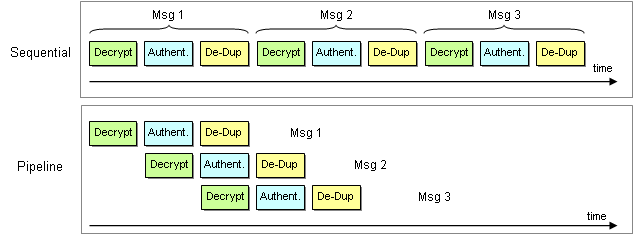
\includegraphics[width=0.8\textwidth]{kuvat/pipeline_processing.png}
      \caption{Kuva sanomien peräkkäisen käsittelyn ja prosessointiputken eroista \citep{Hohpe2004}\label{fig:pipelineprocess}}
      \end{center}
      \end{figure}


      Suodatinketjun suorituskykyä voidaan parantaa tästä entisestään. Edellisessä prosessointiputken esimerkissä heikkoutena on se, että kaikesta hitain suodatinprosessi määrää koko järjestelmän sanomien käsittelytahdin. Tässä tapauksessa hitain suodatin voidaan rinnakkaistaa. Haasteena on varmistaa, että jokaisen sanoman voi käsitellä vain yksi rinnakkaisista suodatinprosesseista. Toinen huomioon otettava aspekti on, että rinnakkaistaminen ei takaa sanomien suoritusjärjestyksen säilymistä. Jos sanomien käsittleyjärjestyksellä on väliä, suodatinprosesseja voi olla vain yksi instanssi. Kolmas haaste on suodattimien tilanhallinta. Tilanhallinta rinnakkaisissa operaatioissa lisää tunnettusti kompleksisuutta, niin suodattimen tilanpalautuminen lähtöpisteeseen operaation valmistuttua yksinkertaistaa huomattavasti suodattimien rinnakkaistamista.
      Kuvan~\ref{fig:parallelprocess} esimerkissä Hohpe ja Woof näyttävät miten salauksen purkamisen \textit{(decrypt)} käytetty suodatin voidaan rinnakkaistaa kolmeksi rinnakkaiseksi prosessiksi, koska purkamisoperaatio on työläin suodattimista \citep{Hohpe2004}. Esimerkissä duplikaattien tarkastus \textit{(de-dup)} on pidetty peräkkäisenä prosessina, koska duplikaattien havaitseminen tarvitsee sanomahistorian hyödyntämistä eli operaatio ei ole tilaton ja sen rinnakkaistaminen on haastavaa. 
      \begin{figure}[h]
      \begin{center}
      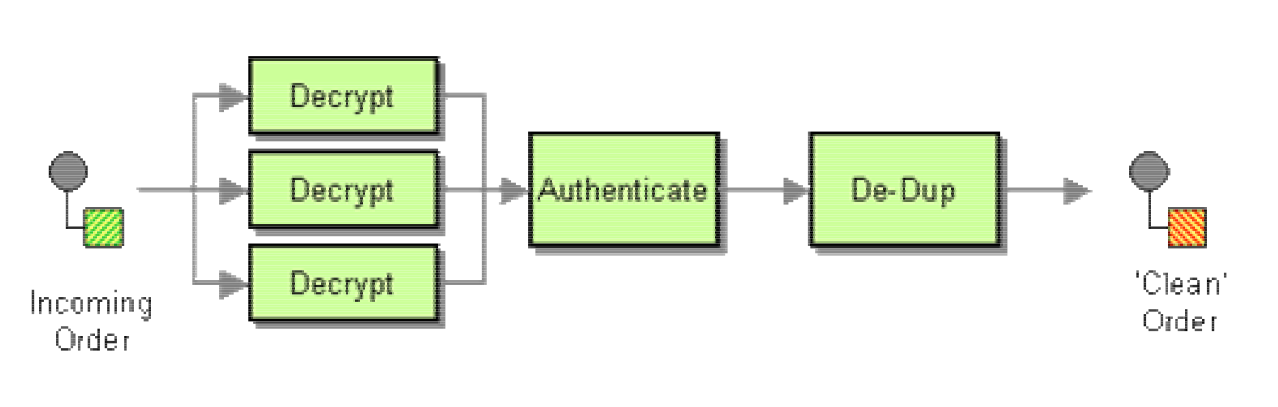
\includegraphics[width=0.8\textwidth]{kuvat/paraller_processing.png}
      \caption{Kuva sanomien rinnakkaisesta käsittelystä kun järjestyksellä on väliä \citep{Hohpe2004}\label{fig:parallelprocess}}
      \end{center}
      \end{figure}


   \item Sanomareititin \textit{(Message Router)}
      Putkien ja suodattimien löyhät kytkennät mahdolistavat uuden prosessointiaskeleen lisäämisen oleamssaolevien väliin. Sanomareitittimen tapauksessa reititin vastaa putkien ja suodattamien suodatinta siinä suhteessa, että se tekee suorittaa prosessointia, mutta suodattimien sijaan reititin on kytketty useampaan ulostulo kanavaan. Reititin ei myöskän muokkaa sanomaa vain on ainoastaan keskittynyt sanomien määränpään valitsemiseen.
   Reitittimen etuna on löyhä kytkentä muihin komponentteihin; ympärillä olevien sudoattimien ei tarvitse olla tietoisia reittittimen olemassaolosta ja kaikki reitityspäätöksien logiikka elää yhdessä sijainnissa. Jos uusia sanomatyppejä tai reititysmuutoksia toteutetaan niin ainoastaan sanomareitittimen logiikka tarvitsee muokata. Koska saapuvan kanavan kaikki viestit siirtyvät reitittimen läpi yksitellen, on saapuvien viestien käsittelyjäjrestys myös taattu.
   Löyhän kytkennän ylläpitohaasteet korostuvat sanomareitintä hyödyntäessä. Jos suurin osa järjestelmästä on löyhästi kytketty toiseen niin järjestlmän kokonaiskuvan muodostaminen käy hankalaksi. Hohpe ja Woofin mukaan näitä haasteita voi lieventää hyödyntämällä sanomien kulkuhistoriaa \citep{Hohpe2004}[sivu~93].


   Reittitimen haasteina ovat erilaiset pullonkaulat. Reittittimestä voi syntyä ylläpidollinen pulonkaula, koska reittittimen pitää olla tietoinen kaikista vastaanottavista kanavista ja tästä voi syntyä ylläpiolline ongelma varsinkin jos vastaanottokanavien lista vaihtuu tiheään. Toinen mahdollinen pullonkaula on suoritysky. Reititin luonteensa vuoksi lisää ylimääräisen prosessointiaskeleen ja monissa sanomajärjestlmissä sanoman siirtäminen toiselle kanavalle vaati sanomien uudelleen koodausta. Useamman reitittimen rinnakkainen käyttö lieventä ongelmaa, mutta jokatapauksessa reititin tulee vaikuttamaan negatiivisesti sanomien viiveeseen vaikka sanomien käsittelytahti pysyisikin samana \citep{Hohpe2004}.
   



\end{itemize}



\chapter{Integraatioteknologioiden jaottelusta}

Laaja-alaisessa tutkimuksessaan \citep{Ritter2017} laajentaa järjestelmäintegraatioiden suunnitelumalleja ja kartoittavat integraatioiden suunnittelumallien käytön kaupallisissa ja avoimen lähdekoodin projekteissa.

Synkrononisia- ja  virtausprotokolleja \textit{(streaming protocol)} ei  ole huomioitu järjestelmäintegraatioisssa eikä niiden suunnittelumalleissa, minkä Hohpe ja Woof myöntävätät \citep{Zimmermann2016}. Erityisesti virtausprotokollien puute aiheuttaa haasteita esimerkiksi big data järjestelmien integraatioissa \citep{Ritter2017}.
Samassa haastattelussa Hohpe Ja Woof toteavatkin, että virtausprotokollien suunnittelumallien dokumentointi parantaisi sanomien käytön ja virtauskäyttötapausten yhtäläisyyksien ymmärtämistä ja johtaisi EIP:een kaltaisten suunnittelumallien löytämiseen \citep{Ritter2017}.

Virtausdatan käsittelemistä EIP-malleilla on kokeiltu laitteistokiihdyttämisen kanssa hyödyntämällä ohjelmoitavia porttimatriiseja \citep{DannRitter2017}. Virtausdatan käsittelyä varten EIP-malleja laajennettiin kahdella uudella suunnittelumallilla: kuormituksen tasaaja \textit{(load balancer)} ja liittäjä reititin \textit{(join router)}. Kuormituksen tasaaja lähettää sanomaan yhteen useasta kanavasta hyödyntämällä yleisiä kuromituksen tasaus mekanismeja. Liittäjä reititin liittää useasta eri kanavasta saapuvat sanomat yhdelle kanavalle ohjelmoidun logiikan mukaisesti.


EIP:een toinen sudenkuoppa on tilalliset \textit{(stateful)} protokollat. Hohpe myöntää, että tilallisesta suunnittelumalleista voisi tulla EIP toinen voluumi ja tilallisten suunnittelumallien sisällyttäminen oikeuttaisi "Enterprise Integrations Patterns" otsikon käyttöä \citep{Zimmermann2016}.
Hohpe on alkanut kerämään tilallisia suunnittelumalleja sivullee \citep{conversationPatterns}, mutta toistaiseksi suunnittelumallit eivät ole poikeneet uutta kirjaa. Verrattuna EIP:een Hohpen tilalliset mallit käyttävät sanomien sijaan keskusteluja \textit{(conversations)} jonka ympärille suunnittelumallien abstarktiot on rakennettu.



Virheenhallinnasta:
To handle erroneous situations during message processing, escalate them and make systems more fault-tolerant, error handling is seen as a major aspect [5], [45]. Hohpe et al. [3], [70] do only cover Dead Letter Channel as solution and sketch some ideas about the topic. Overall, in the literature, the topic is neither addressed from a pattern, formalization, nor modeling perspective. While [5] mentions missing patterns and formalization, Merkel et al. [45] lists Balancing and Distribution, as well as [69] mentions Fault-tolerance and Message Scheduling as missing aspects. Similarly, the insight into the current state of affairs, called monitoring, for services and cross-cloud are seen as important topics in [45], [61], [62]\citep{Ritter2017}




\chapter{Yhteenveto}
